\chapter{Boson simulations}
\label{ch:Simulations}
In this chapter I discuss two instances of linear optical quantum simulations.
The first is a full simulation of the time evolution of vibrational excitations
in molecules. This work is being prepared for publication in \cite{molecules},
with co-authors Enrique Mart\'in L\'opez, Chris Sparrow Jeremy O'Brien and
Anthony Laing. Some material appears in Enrique's PhD thesis \cite{enrique}. The
physical platform used in this simulation was a bulk optics circuit built by
Enrique, which I calibrated. The experiment was planned by Enrique and the
overall project was supervised by Anthony. Data was collected by me and Chris
Sparrow and analysed by me.

The second simulation moves away from closed quantum systems obeying Hermitian
dynamics and considers a more abstract system of bosons obeying (non-Hermitian) 
PT-symmetric dynamics. This work is being prepared for publication in
\cite{pt-prep} with co-authors Yogesh Joglekar, Chris Sparrow, Chris Harrold,
Jeremy O'Brien and Anthony Laing. The theory for this section (the
\(\pt\)-symmetric model) was developed by Yogesh and I planned the experiment.
Two physical platforms were used: the bulk optics circuit used for the molecules
experiment and a larger integrated circuit. Data on the bulk circuit was taken
by me and Chris Sparrow; Chris Harrold took data on the integrated circuit.

\section{Introduction}
\label{sec:SimIntro}
Simulation of quantum systems, for example calculation of the electronic energy
states of molecules,
is a major challenge for classical computers, with even the fastest algorithms
falling short of polyomial scaling with the system size. Approximations can be
pretty good, but cases such as the simulation of catalyst molecules, fall short
of the required precision for useful theoretical conclusions. \todo{This is
mostly based on the presentation at Microsoft - find some citations.} A solution
was proposed by Feynman \cite{qsim-feynman} in the early days of quantum
information science: use a quantum system to simulate other quantum systems.
Further study of quantum computing has formalised this idea and we now
understand that if we had sufficient control over one non-trivial quantum systemto build a universal quantum computer, we could program it to simulate any other
quantum system.

I will refer to this method of simulation as \emph{digital} quantum simulation,
since it translates the dynamics of the simulated system into operations on
qubits: digital quantum information. The main advantage of digital simulation is
that it is implemented on a quantum computer, for which error correcting
algorithms provide a path for scalability. A further advantage is that
algorithms can be devised independently of the physical system implementing the
qubits, which could be anything from trapped ions to guided photons. Indeed,
simulations of small molecules have been performed on such diverse platforms as
linear optics~\cite{qsim-peruzzo} and NMR~\cite{qsim-du}. \todo{and others?}
However these advantages are currently offset by the large resource overheads
required for the encoding. While some progress has been made in reducing the
overheads~\cite{qsim-poulin}, like any application involving digital quantum
computing, the technical challenge remains formidable.

An alternative approach to quantum simulation is the \emph{analogue} simulator.
While digital quantum simulation can be compared to modelling planetary motions
on a classical computer, analogue simulation bears more resemblance to an
orrery: a mechanical system that actually moves models of the planets. This may
seem like a primitive approach to simulation, but it has the advantage of
leveraging properties of the simulator to reduce the overheads in performing the
simulation (at the cost of abandoning known methods for error correction) and
may be a quicker route to outperforming classical algorithms
\cite{qsim-analogue}. In
this chapter, I discuss how to take advantage of the properties of photons in
linear optics to perform simulations of other systems of non-interacting bosons
without the overheads of a universal quantum computer.

By way of introduction, consider four broad categories of quantum objects.
First, group by exchange symmetry: fermions and bosons, then by interactions:
particles can interact with each other (e.g. charged particles via the
electromagnetic force) or not. Full simulation of arbitrary interacting systems
is believed to have the same requirements as a general quantum computer. When
interactions can be ignored, we have a much more limited simulator, and if we
are further restricted to non-interacting fermions, the system can be simulated
classically \todo{citation needed}. The final category---non-interacting
bosons---is likely to yield more interesting results and since the recent
proposal of \bosonsampling{}~\cite{bosonsampling} appears to be intractable to
classical simulation under certain conditions.

Photons belong to this final class: they are bosonic particles, and infamously
non-interacting (proposals for universal photonic quantum computers rely on
effective interactions via detection~\cite{klm}). The implication of this is
that with a relatively simple quantum computer (a system of photons in a large
interferometer) we can go beyond the original \bosonsampling{} algorithm and
perform meaningful quantum simulations.

\section{Experimental Setup}
\subsection{Bulk Optics}
\label{sec:BulkReck}
\begin{figure}[t]
  \centering
  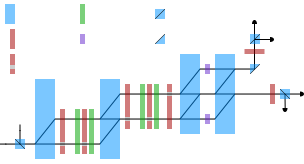
\includegraphics{figures/circuit.pdf}
  \caption[A schematic of the bulk optics circuit used for simulations.]
  {A schematic of the bulk optics circuit. Two photons are injected at
  the left of the circuit in orthogonal polarisations (\(\ket{H}\) indicates
  horizontal and \(\ket{V}\) indicates vertical), using an in-fibre polarising
  beamsplitter (PBS) to combine the two photons into a single path. The circuit
  operates in a combined path/polarisation encoding, where polarising beam
  displacers (PBD) are used to convert between the two. Operations are performed
  with fixed quarter waveplates (QWP) and polarisation flips (X), and variable
  angle half waveplates (HWP). After the operations are complete,
  polarisation-sensitive detection is performed using further PBS elements and
  single photon avalanche diodes. We label the detectors A through D.}
  \label{fig:circuit}
\end{figure}
The results in this chapter were obtained using the bulk optics circuit shown in
figure~\ref{fig:circuit}. This circuit allows complete reconfigurability and
arbitrary control over two photons in four optical modes. Operationally, it is
similar to the scheme in~\cite{reck} (introduced in
section~\ref{sec:ReckScheme}), but architecturally it is optimised for a stable
implementation in bulk optics using combined path/polarisation encoding and 
Jamin-Lebedef interferometers. Reconfigurability is provided by a series of 7
half waveplates, 5 of which give control over the amplitude splitting of the
photons with the remaining 2 controlling the internal phases. Since we always
inject and measure in the computational basis (i.e.\ exactly one photon in each
input mode and no interferometry at the output) there are 4 phases that would
appear in a general unitary but which do not affect our results, plus a global
phase that would not be detected by any experiment. More detail on the
calibration of the circuit is provided in chapter~\ref{ch:QCV}.

Up to two photons can be injected at the input, initially in orthogonal
polarisations, \(\ket{H}\) and \(\ket{V}\). The operation performed on the
photons' state is described by a \(4 \by 2\) unitary (only 2 columns are
required because there are only 2 inputs),
\begin{align}
  \mat{U} = \begin{pmatrix}
    q_{0} & t_{0} \\
    q_{1} & t_{1} \\
    q_{2} & t_{2} \\
    q_{3} & t_{3}
  \end{pmatrix} && \begin{array}{l}
    U \ket{V} = \ket{\vec{q}} \\
    U \ket{H} = \ket{\vec{t}}
  \end{array}
\end{align}
We refer to the final state of the photon injected in the \(\ket{V}\) mode as
the \emph{quart} and the final state of the photon injected in the \(\ket{H}\)
mode as the \emph{trit}. At the end of the circuit we detect photons in each of
the four modes. We can perform either single photon counting or photon
coincidence detection.

The reconfigurability of our circuit is obtained by joint path/polarisation
operations. We can control the amplitudes at the output with half waveplates
(HWPs), and the phases with a series of three waveplates (QHQ): a half waveplate
between two quarter waveplates with the optic axis orientated at 45 degrees.
We use beam displacers (BDs) to convert between path and polarisation and
implement very stable Jamin-Lebedeff interferometers, while
polarisation-sensitive detection is achieved with in-fibre polarising
beamsplitters (PBS) and single-photon avalanche diodes (SPADs).

\subsection{Integrated platform}
This is realised in integrated optics, using thermo-optic phase shifts and Mach
Zehnder interferometers (MZIs) to achieve the necessary reconfigurability.
\todo{Describe the integrated Reck scheme here.}

\section{Data Analysis}
\subsection{Presentation of Data}
\todo{This is where I explain which modes I am presenting, and how we have
`saturated the distribution'---not a scalable approach. Maybe also the time to
mention the scale factor in \(\pt\) section.}

\subsection{Figures of Merit}
\todo{Move any definition of figures of merit (trace distance and Kolmogorov
distance here.}

To evaluate the fidelity of our simulations, we look at two measures. The first
is a trace distance between the unitary matrix that we intended to implement,
and the matrix that we in fact did implement, according to the data we collect
\cite{sst}. If the desired unitary is \(\mat{U}\) and the measured unitary
is \(\mat{U^{\prime}}\), the trace distance, \(F\) is defined by:
\[F=\frac{1}{2}\Tr\of{\mat{U}^{\dagger}{\mat{U}^{\prime}}}\]
The second measure we use compares (normalised) discrete probability
distributions, \(p\) and \(q\). This fidelity is computed as:
\[F=1-\frac{1}{2}\sum_{i}\abs{p_{i}-q_{i}}\]
This can be computed for the single photon data without any normalisation, since
detection probabilities in the four modes \(S_1\),\(S_2\),\(E_1\) and \(E_2\)
must sum to 1. In the case of coincidences, we only measure 6 out of the 10
possible pairings, so we must normalise these to 1 before computing the
fidelity.

\section{Molecular Vibrations}
\label{sec:Molecules}
\begin{figure}[h]
  \centering
  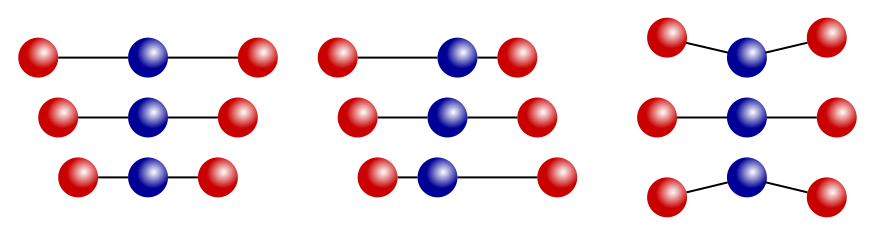
\includegraphics{figures/vibrations.pdf}
  \caption[Vibrational modes of linear triatomic molecules]
  {Illustration of the vibrational modes of linear triatomic molecules. (a)
  Symmetric stretch, (b) Asymmetric stretch, (c) Bend. There are two
  (degenerate) bending modes, one in each of the two directions perpendicular to
  the axis of the molecule. In each case, the middle row shows the equilibrium
  positions of the atoms and the diagrams either side show the extremes of the
  motion.}
  \label{fig:vibrations}
\end{figure}
In this section I present results from the quantum simulation of quantized
vibrations in molecules. The theory was developed by Enrique Mart\'in L\'opez
and the overall project was supervised by Anthony Laing. I was responsible for
the calibration of the circuit, taking part of the data (for the OCS moleculels)
and analysis of the data. The rest of the data (the \co{} molecules) was taken
by Chris Sparrow, who I instructed in the use of the circuit.

\subsection{Introduction to phonons}
\label{sec:Phonons}
In classical physics, systems of coupled oscillators can be analysed in terms of
their normal modes, representing collective motions of the individual
oscillators with well-defined frequencies. If the magnitude of the oscillation
is large, the excitation of one normal mode can shift the frequency of other
normal modes, a kind of interaction. However, in the limit of small
oscillations, this shift vanishes and the normal modes do not interact. We call
this the harmonic limit.

In quantum mechanics, a system of coupled oscillators (like any other system)
can be described by its Hamiltonian. The Hamiltonian can be diagonalised,
yielding the eigenstates of the system, equivalent to the normal modes of a
classical oscillator. We can define creation and annihilation operators for
excitations of the eigenstates, and treat them as bosonic quasiparticles:
phonons. In the harmonic limit, these phonons do not interact, and can thus be
simulated by our system.

\subsection{Application to Molecules}
In the bulk optics circuit we have four optical modes, which allows us to
simulate 4-level molecules
exactly. In general, a completely asymmetric \(n\)-atom molecule will have \(3
n-6\) vibrational states (the remaining 6 degrees of freedom are
uniform translation in three directions and rotation about three axes). A linear
molecule has rotational symmetry about one axis; in this case the rotational
mode about this axis of symmetry is composed of (degenerate) bending modes and
there are \(3n - 5\) vibrational modes. Therefore a linear 3-atom molecule will
have four vibrational modes, making it a suitable candidate for simulation in
our system. The four modes are illustrated in figure~\ref{fig:vibrations}.

We identify two such molecules to simulate: carbon dioxide (\co{}) and carbonyl
sulphate (OCS). The energies of the vibrational modes are taken from
spectroscopic data on the HITRAN database~\cite{hitran}, to give us the
Hamiltonians in the diagonal basis:
\begin{align}
  H_{\text{OCS}} = \begin{pmatrix}
    520 & 0 & 0 & 0 \\
    0 & 520 & 0 & 0 \\
    0 & 0 & 859 & 0 \\
    0 & 0 & 0 & 2062 \end{pmatrix} && , && H_{\text{CO}_{2}} = \begin{pmatrix}
    667 & 0 & 0 & 0 \\
    0 & 667 & 0 & 0 \\
    0 & 0 & 1388 & 0 \\
    0 & 0 & 0 & 2349 \end{pmatrix}
\end{align}
in units of \(\cm^{-1}\). This is sufficient information to perform simulations
of the evolution of the vibrational state of the molecules.

\begin{figure}
  \centering
  \includegraphics{figures/molecules}
  \caption[Simulation of quantized vibrational states in molecules]
  {Simulation of quantized vibrational states in molecules. Blue is \co{} and
  green OCS. Lines represent the theoretically calculated evolution of the
  probabilities, with shaded regions showing \(\pm 1 \sigma\) expected due to
  errors in dialling. Points are experimentally measured, with error bars due to
  Poissonian noise too small to see at this scale.}
  \label{fig:molecules}
\end{figure}

The only aspect of the simulation to be determined is the preparation and
measurement basis. If we prepare or measure in the any of the eigenmodes, the
time evolution will be trivial; more interesting simulations are derived when
the preparation and measurement basis both differ from the diagonal basis.
Suppose that the unitary
operators mapping the computational basis to the preparation and measurement
bases are \(\mat{V}_{\prep}\) and \(\mat{V}_{\meas}\), respectively. Then the
unitary operator describing the evolution of
the state for a time \(t\) is:
\begin{equation}
  \mat{U} \of{t} = \mat{V}_{\meas}^{\dagger} \cdot e^{-i \mat{H} t/\hbar} \cdot
  \mat{V}_{\prep}
\end{equation}
This expression can be understood as mapping the computational state at the
input to the device onto one of the preparation basis states, then performing
the time evolution in the diagonal basis and finally projecting from a
measurement basis state back onto the computational basis measured by our
detectors. We chose the measurement and preparation bases randomly and
independently, according to the Haar measure since this brings us into the
regime described by \bosonsampling{}: while the \(\mat{U} \of{t}\) and \(\mat{U}
\of{t^{\prime}} \) will be correlated, any individual instance will be a Haar
random unitary.

\subsection{Results}
Given a diagonal Hamiltonian and preparation and measurement bases, we proceed
with the simulation using a discrete time method. We dial \(\mat{U} \of{t}\) for
21 values of \(t\) equally spaced in the interval \(\left[0,0.01\right]\)
(units of \(\cm / c\)) and record single-phonon occupations and
phonon-pair coincidences at each time. The results are shown in
figure~\ref{fig:molecules}.

\todo{Summarise fidelities across the simulation. Table?}

\section{PT-symmetric systems}
\label{sec:PT}
The simulations presented in the previous section are entirely concerned with a
closed quantum system, evolving according to Hermitian dynamics. I now turn my
attention to quantum systems described by non-Hermitian Hamiltonians,
particularly those that are invariant under the combined parity \((\op{P})\) and
time-reversal \((\op{T})\) operations.

Systems obeying \(\pt\) symmetry have been theoretically explored for more than
a decade \cite{bender98, levai-jphysa-33-7165, bender07}. Although not
Hermitian, the Hamiltonians have a purely real spectrum that changes into
complex-conjugate eigenvalues as the non-Hermiticity is increased. When the
spectrum of \(\mat{H}_{\pt{}}\) is purely real, its non-orthogonal
eigenvectors are simultaneous eigenvectors of the \(\pt{}\) operation. However,
when the spectrum has complex conjugate eigenvalues, due to the anti-linear
nature of the operator \(\op{T}\), the eigenvectors are not \(\pt{}\)
symmetric. This transition from real to complex spectrum is called \(\pt{}\)
symmetry breaking. 

It has been established that \(\pt{}\) symmetric theory is unlikely to be a
complete alternative to quantum mechanics, either reducing to the same thing
\cite{mostafazadeh-jmathphys-43-205} or producing non-physical results such as
violation of the no-signaling principle of relativity \cite{lee-prl-112-130404}.
However, it has recently become clear that it is far from being just a
mathematical curiosity: \(\pt{}\)-symmetric Hamiltonians model open
systems---classical or quantum---with balanced, spatially separated loss and
gain. They have been used to theoretically investigate vortex hopping in
superconductors \cite{naomichi-physrevlett-77-570},
statistical mechanics of Coulomb gases \cite{gulden-jetp-117-517} and
non-equilibrium superconductivity \cite{rubinstein-physrevlett-99-167003,
serbyn-physrevb-87-020501}. In recent years, the \(\pt{}\)
symmetry breaking has been experimentally investigated in classical systems
including two optical waveguides \cite{pt-ruter}, electrical circuits
\cite{schindler-physreva-84-040101}, mechanical systems
\cite{bender-amjphys-81-173} and discrete fiber networks
\cite{pt-regensburger}.

I will now demonstrate the quantum simulation of non-interacting bosons
evolving under a \(\pt{}\) symmetric
Hamiltonian. We investigate the single-particle statistics and bosonic
correlations across the \(\pt{}\) symmetry breaking threshold. Although the time
evolution under \(\mat{H}_{\pt{}}\) is not unitary, by embedding this open
system into a larger, closed system, we demonstrate a general method for
simulating non-Hermitian Hamiltonians.

\begin{figure}[t]
  \centering
  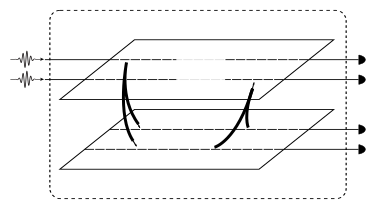
\includegraphics{figures/opensystem}
  \caption[Representation of an open system]
  {Schematic representation of a simulation of an open system. We initialise a
  state in the system subspace, which then evolves under a non-Hermitian
  Hamiltonian to occupy a larger space. Detection on all output modes can reveal
  information about evolution into the environment subspace.}
  \label{fig:opensystem}
\end{figure}

\begin{figure}[t]
  \centering
  \includegraphics{figures/manifolds}
  \caption[Manifolds showing evolution of the PT-symmetric system]
  {Manifolds showing evolution of the \(\pt{}\)-symmetric system. In each case,
  the state is initialised with a single excitation in the system loss mode
  \(S_{0}\). The time evolution of the occupation of mode \(S_{0}\) is shown
  for a range of \(\gamma\), where \(\gamma < 1\) is the \(\pt\) symmetric
  region and \(\gamma > 1\) is the \(\pt\) broken. Lines show the values of
  \(\gamma\) (0.95,1.0,1.05) that we have used in the experiment. In (a)
  unnormalised occupations are shown on a logarithmic scale, while in (b) the
  occupations have been normalised and experimental data are shown as points.}
  \label{fig:manifolds}
\end{figure}

\subsection{Two-site PT-symmetric model}
Let us consider a 2-site Hamiltonian with a tunneling \(J > 0\) between the two
sites and a \(\pt{}\)-symmetric potential \(\pm i \gamma\) on the two sites, \(
\mat{H} = -J \sigma_x -i \gamma \sigma_z\). The eigenvalues of this matrix are
\( \epsilon = \pm \sqrt{J^{2} - \gamma^{2}} \) which are real for \( J \geq
\gamma \), although the eigenvectors are not orthogonal to each other.

First, let us assume that the non-Hermitian term is small, i.e. \( \gamma \leq
J \) and \( \epsilon \) is real. In this case, we get the following
(non-unitary) time-evolution operator with \( \alpha = \epsilon \frac{t}{\hbar}
\)
\begin{equation}
  \mat{G}_{\leq} \of{t} = \begin{pmatrix}
    \cos \alpha - \frac{\gamma}{\epsilon} \sin \alpha &
    i \frac{J}{\epsilon} \sin \alpha \\
    i \frac{J}{\epsilon} \sin \alpha &
    \cos \alpha + \frac{\gamma}{\epsilon} \sin \alpha
  \end{pmatrix}
\end{equation}

In the limit where \( \gamma \rightarrow J_{-} \), \( \epsilon \rightarrow 0 \)
and \( \frac{1}{\epsilon} \sin \alpha \rightarrow \frac{t}{\hbar} \), thus at
the \(\pt{}\) phase boundary the time evolution operator becomes linear in time
instead of sinusoidal:
\begin{equation}
  \mat{G}_{\leq,-} = \begin{pmatrix}
    1-J\frac{t}{\hbar} & i J\frac{t}{\hbar} \\
    i J\frac{t}{\hbar} & 1+J\frac{t}{\hbar}
  \end{pmatrix}
\end{equation}
This also follows from the fact that \( \mat{H}^{2} = 0\) when \(J = \gamma\),
thus \( \mat{G}_{\leq} \of{t} \) truncates to the first two terms.

If we allow a large non-Hermitian term, \( \gamma \geq J \), then the
eigenvalues are purely imaginary, \( \epsilon = \pm i \sqrt{ \gamma^{2} - J^{2}
} = i \Gamma \). The corresponding eigenvectors are still not orthogonal. In
this case, the time evolution operator (with \( \beta = \Gamma \frac{t}{\hbar}
\)) is
\begin{equation}
  \mat{G}_{\geq} \of{t} = \begin{pmatrix}
    \cosh \beta - \frac{\gamma}{\Gamma} \sinh \beta &
    i \frac{J}{\Gamma} \sinh \beta \\
    i \frac{J}{\Gamma} \sinh \beta &
    \cosh \beta + \frac{\gamma}{\Gamma} \sinh \beta
  \end{pmatrix}
\end{equation}
In the limit where \( \gamma \rightarrow J_{+} \), \( \Gamma \rightarrow 0 \)
and \( \frac{1}{\Gamma} \sinh \beta \rightarrow \frac{t}{\hbar} \) thus at the
\(\pt{}\) phase boundary, we get a continuous time evolution operator,
\begin{equation}
  \left. \mat{G}_{\leq} \of{t} \right|_{\gamma \rightarrow J_{-}} = \left.
    \mat{G}_{\geq} \of{t} \right|_{\gamma \rightarrow J_{+}}
\end{equation}

The behaviour of this \(\pt{}\)-symmetric system can be understood by looking at
the occupation of (system or environment) modes when a particle initially in the
system is evolved under the non-Hermitian \(\mat{H}\). This will be a function
of the ratio \(\gamma/J\) as well as the time. In figure~\ref{fig:manifolds} we
illustrate this by setting \(J=1\) and showing the occupation of one of the
system modes as a function of time for a range of values of \(\gamma\). The
transition from \(\pt{}\) symmetric to \(\pt{}\) broken can be seen, and the
occupations are continuous over the boundary. Also shown are cross-sections
where experimental data are taken (see figure~\ref{fig:twosite} for full
experimental data).

\subsection{Three-site PT-symmetric model}
\label{sec:ThreeSite}
We can expand this model to a 3-site system, where the Hamiltonian is given by:
\begin{equation}
  \mat{H}_{3} = \begin{pmatrix}
    i \gamma & -\eta & 0 \\
    -\eta & 0 & -\eta \\
    0 & -\eta & -i \gamma \\
  \end{pmatrix} = \mat{H}_{3}^{\transpose} \neq \mat{H}_{3}^{\dagger}
\end{equation}
When \(\gamma=0\), this is familiar in a photonics context as a
continuously-coupled quantum walk on three modes with uniform coupling between
the modes. The eigenvalues are \(\left\{ -\sqrt{2} \eta, 0 +\sqrt{2}
\eta\right\}\), and the eigenvectors are orthonormal.

In the case \(\gamma \neq 0\), the matrix is no longer Hermitian. Physically,
the scenario describes a gain on mode 0 and an equal loss on mode 2, while
mode 1 remains lossless. The eigenvalues are now \(\left\{ \pm \sqrt{2 \eta^{2}
- \gamma^{2}}, 0 \right\}\), and we observe the same \(\pt\) symmetry breaking
as in the two-site model. When the non-Hermitian term is sufficiently small
(\(\gamma \leq \sqrt{2} \eta\)), the spectrum is real, while above this
threshold (\(\gamma > \sqrt{2} \eta\)), we see a pair of complex conjugate
eigenvalues emerge. The behaviour of the system is again continuous across the
\(\pt\) boundary.

\subsection{Unitary Dilation}
The simulation technique that we use requires that we embed the non-unitary
time-evolution operator into a larger, unitary operator. This can be done for
any matrix by doubling the dimension; that is, any \(n \by n\) matrix can be
embedded as an \(n \by n\) submatrix of a \(2n \by 2n\) unitary matrix. In order
to perform this embedding for a non-unitary matrix \(\mat{G}\), we must first
rescale it so that the operator norm is less than or equal to 1. A suitable
definition of operator norm in this case is \(\abs{\mat{G}} = \sqrt{\abs{e_{
\text{max}}}}\), where \(e_{\text{max}}\) is the largest eigenvalue of 
\(\mat{GG^{\dagger}}\) \cite{dilation}. The scaled matrix is then
\begin{equation}
  G_{s} = \frac{G}{\sqrt{\abs{e_{\text{max}}}}}
\end{equation}
and the unitary dilation can be expressed as follows:
\begin{equation}
  U = \begin{pmatrix}
    \mat{G}_{s} & \mat{D}\of{\mat{G}_{s}} \\
    \mat{D}\of{\mat{G}_{s}^{\dagger}} & -\mat{G}_{s}^{\dagger} \end{pmatrix}
\end{equation}
where \(\mat{D}\of{\mat{G}_{s}} = \left( \identity - \mat{G}_{s}\mat{G}_{s}^{
\dagger} \right)^{\half}
\) is the \emph{defect matrix} of \(\mat{G}_{s}\).

It can be verified by explicit calculation that \(\mat{U}\) is unitary.
Since \(\mat{G}_{s}\mat{G}_{s}^{\dagger}\) is always Hermitian, it always has
real eigenvalues and thus the defect matrix is well defined.

Physically, the interpretation of this unitary matrix corresponds to doubling
the number of available modes by introducing an \emph{enviroment} space, of
equal dimension to the \emph{system}. The rationalisation for this increase in
size being sufficient is that each system mode needs only one loss/gain channel
to realise arbitrary dynamics: adding more does not provide any additional
freedom.

The top left corner contains the matrix \(\mat{G}_{s}\), which describes
dynamics within the system and the bottom right corner
(\(-\mat{G}_{s}^{\dagger}\)) describes dynamics within the environment.
Since \(\mat{G}_{s}=\exp \of{-i\mat{H}t/\hbar}\), the evolution of the
environment, \(\mat{-G}_{s}^{\dagger}=-\exp \of{i\mat{H}t/\hbar}\) is the
time-reversal of the system's evolution (with a constant phase). The cross
terms, \(\mat{D} \of{\mat{G}_{s}}\) and \(\mat{D} \of{\mat{G}_{s}^{ \dagger}}
\), describe the coupling between the system and environment. If
\(\mat{G}_{s}\) is already unitary, this coupling disappears, as expected:
unitary evolution applies to a closed system.

A consequence of this simulation method is that there is no effective
Hamiltonian that models the evolution of the closed system, i.e. no matrix
\(\mat{H}_{\eff}\) can satisfy
\begin{equation}
  U\of{t} = e^{-i\mat{H}_{\eff}t/\hbar}
\end{equation}
for all times \(t\). This is evident when considering the initial time \(t=0\).
We would require
\begin{equation}
  \mat{U}\of{0} = \begin{pmatrix}
    \identity & 0 \\
    0 & -\identity
  \end{pmatrix}
\end{equation}
which cannot be achieved for any effective Hamiltonian. This observation implies
that the environment modes introduced for the simulation do not really
correspond to a real physical system; rather they are just a convenient way of
keeping track of gain and loss.

\begin{figure}[p]
  \centering
  \includegraphics{figures/twosite}
  \caption[Results of simulation]
    {Results of our experimental simulation. The top row (a-c) shows
    single photon data. The photon is initially injected in the system mode
    \(S_1\); probability of detection in each of the four modes \(\left\{S_1,
    S_2, E_1, E2\right\}\) after the evolution is shown. (a) is in the
    \(\pt{}\)-symmetric region (\(\gamma=0.95\)), where we observe periodic
    behaviour. (b) is on the \(\pt{}\) phase boundary (\(\gamma=1\)) and (c) is
    in the \(\pt{}\) broken region (\(\gamma=1.05\)). In both of these cases,
    the detection probabilities in our
    experiment tend towards a constant value, with any evolution after this
    point being purely due to the scale factor. The bottom row (d-f) shows
    two-particle data, where the particles are initially injected in the two
    system modes, \(S_1\) and \(S_2\). We show the detection probabilities for
    pairs where one photon is still in mode \(S_1\), and the other photon is in
    a different mode. (d) is in the \(\pt{}\)-symmetric region
    (\(\gamma=0.95\)), and again exhibits periodic behaviour. (e) is on the
    \(\pt{}\) phase boundary (\(\gamma=1\)) and (f) is in the \(\pt{}\)-broken
    region (\(\gamma=1.05\)). In all cases, the scale factor (black dashed
    line; on a different axis), has been separated out from the experimental
    observations, which reflect detection probabilities, rather than mode
    occupation.}
  \label{fig:twosite}
\end{figure}

\subsection{Four Mode Simulation}
\label{sec:FourMode}
For our simulation we use a reconfigurable, four-mode photonic circuit in bulk
optics, shown in figure~\ref{fig:circuit}. We map two of these optical
modes to the system and two to the environment, so the transformation performed
by the circuit is guaranteed to be unitary. By looking at detection events on
only the system modes, \(S_1\) and \(S_2\) we can observe (a scaled version of)
the evolution of the \(\pt{}\)-symmetric system, or by considering detection
events on any other modes, we can study the interaction between the system and
the environment. Note that when post-selecting on the system modes, there is a
non-unit probability of a detection event. In light of this, we could not
simulate the super-luminal signalling described in \cite{lee-prl-112-130404}.

The graphs in figure~\ref{fig:twosite} show the evolution of the 2-site system
at 3 points in the parameter space: \(\pt{}\)-symmetric, \(\gamma=0.95\) (a,d);
\(\pt{}\)-critical, \(\gamma=1.0\) (b,e) and \(\pt{}\)-broken, \(\gamma=1.05\)
(c,f). The scale factor (i.e. operator norm of the non-unitary matrix) has been
seperated from the experimental data for clarity. Consequently, the occupation
probabilities are always bounded between zero and one, and reflect the
probabilities of detecting photons in the relevant optical modes. On the other
hand, the scale factor is unbounded, and this is the origin of the quadratic or
exponential growth in the critical and \(\pt{}\) broken regions.

The top row (a-c) shows single-photon data, where the photon is injected into
system mode \(S_1\). Occupation probabilities for all output modes are shown.
The bottom row shows coincidental detections, where the photons are injected
into the two system modes, \(S_1\) and \(S_2\). We show occupation probabilities
for one photon in system mode \(S_1\) and the other photon in a different mode.
In both the \(\pt{}\)-critical and \(\pt{}\)-broken regions, the coincidental
detections between system and environment have very low probability.

Throughout all graphs, points represent experimental data (error bars due to
Poissonian noise are too small to see at this scale) and lines represent
theoretical expectations. The dashed black line (not on the same scale) is the
scale factor, and is unbounded.

In summary, the fidelities obtained are \(0.948 \pm 0.052\) for the trace
distance, \(0.956 \pm 0.020\) for the single photon data shown and \(0.961 \pm
0.014\) for the coincidences. Note that the figure for the coincidences takes
into account the \(S_2 E_1\), \(S_2 E_2\) and \(E_1 E_2\) correlations, which
are not presented here.

\subsection{Six Mode Simulation}
\label{sec:SixMode}
In order to perform a simulation of the three-site \(\pt\)-symmetric model using
the method of unitary dilation, we require an optical circuit with six modes.
Full simulations of the time evolution are performed for two regions of the
phase space: one below and one above the \(\pt\) threshold. The results of the
simulation can be seen in figures~\ref{fig:threesitesingles} (single photon
data) and~\ref{fig:threesitetwofolds} (two photon correlations).
\begin{figure}[p]
  \centering
  \includegraphics{figures/threesite_singles}
  \caption[Single photon data from simulation of the 3-site PT symmetric model]
  {Single photon data from simulation of the 3-site \(\pt\) symmetric model}
  \label{fig:threesitesingles}
\end{figure}

\begin{figure}[p]
  \centering
  \includegraphics{figures/threesite_pairs}
  \caption[Two photon data from simulation of the 3-site PT symmetric model]
  {Two photon data from simulation of the 3-site \(\pt\) symmetric model}
  \label{fig:threesitetwofolds}
\end{figure}

The fidelities are calculated using the Kolmogorov distance between two
normalised probability distributions, and summarised below:

\begin{tabular}{|l|l|l|l|}
  \hline
  \multicolumn{2}{|c|}{Symmetric} & \multicolumn{2}{|c|}{Broken} \\
  \hline
  Singles & Twofolds & Singles & Twofolds \\
  \hline
  \(0.96 \pm 0.03\) & \(0.98 \pm 0.02\) & \(0.96 \pm 0.02\) &
  \(0.98 \pm 0.02\) \\
  \hline
\end{tabular}

\section{Conclusions}
In this chapter I have demonstrated the power of linear optics to bosonic
excitations in a wide variety of settings. The simulations of vibrational states
in molecules shows an application to a system of genuine practical use,
which is beginning to attract wider interest from the physical chemistry
community \cite{vibronics}. I have also shown how, with a modest increase in
experimental complexity, open quantum systems can be simulated with the same
techniques. The procedure employed here generalises beyond the \(\pt\)-symmetric
systems studied, to any non-Hermitian dynamics of non-interacting bosons. While
\(\pt\)-symmetric systems have been studied experimentally in the past, the
results presented here are arguably the first fully quantum simulations,
compared to (for example) coherent light in \cite{pt-ruter} and
\cite{pt-regensburger}.

By going from a bulk optics circuit to an integrated platform, I have
demonstrated a path to scalability for this kind of simulation. There are no
clear fundamental obstacles to increasing the size of integrated optics circuits
to thousands of optical modes, while classical simulations would break down long
before this. Overall, I conclude that analogue quantum simulation has the
potential to outperform classical computers before large scale digital quantum
simulation becomes practical.

\section{Experimental details}
\label{sec:SimulationExperiment}
\subsection{Four mode circuit in bulk optics}
The circuit shown in figure~\ref{fig:circuit} can be used to realise any
unitary operator in 4 modes, down to experimentally undetectable phases on the
input and output modes. This insensitivity to certain phases reduces the number
of parameters that we need to control to 7. All of the tunable parameters are
realised experimentally with half waveplates (HWPs), 5 of which control
amplitude splitting and the remaining 2 control internal phases
(interferometers). The calibration of the circuit is decribed in
section~\ref{sec:Calibration} of chapter~\ref{ch:QCV}.

The type-I spontaneous parametric down-conversion source used a 404nm
continuous-wave laser focused to a 40 \(\mu\)m waist in a \(\text{BiB}_3
\text{O}_6\) (Bismuth Triborate) non-linear crystal to produce pairs of
degenerate photons at 808nm. The photon pairs were filtered with high
transmission interference filters of 3nm spectral width and collected into
polarisation-maintaining optical fibres. Single-photon detection was achieved
using silicon-based avalanche photodiode single-photon counting modules.
Coincidence counting logic used a field-programmable gate array.

\subsection{Six mode circuit in integrated optics}
For the three-site \(\pt\)-symmetric model, we require six optical modes to
simulate the non-unitary evolution in three modes. A fully reconfigurable
circuit in integrated optics is used for this purpose.

\subsection{Data acquisition}
For each unitary operator that we implement, we take one- and two-photon data.
The one-photon data are obtained by injecting one photon into the circuit, with
the other photon from the created pair acting as a herald, and counting
coincidental detections between them. An integration time of 30 seconds is used
for each of the two input modes ofthe circuit.
% NOTE: Remember that we take the one-photon data with 4 detectors, so we first
% herald with detector A and measure BCD and then herald with detector D and
% measure ABC.
The two-photon data consist of injecting both photons simultaneously then
delaying one photon from the pair with respect to the other to observe the
quantum to classical transition in photon correlations. This is done for each
pair of different output ports giving a total of six pairwise data sets in our
four-mode case. Two-photon data points were taken every 0.02mm over a range of
0.48mm with 20 seconds integration time.

Finally, we measure the relative detector efficiencies for the circuit. To do
this, we inject unheralded photons from one arm of the source through the input
mode \(S_1\), and direct them to each of the output ports in turn. The ratios of
counts at each of detectors \(S_2\), \(E_1\) and \(E_2\) to the counts at
detector \(S_1\) (after an integration time of 20 seconds and subtracting the
background of dark counts) give us the relevant efficiency data. We use this
measured efficiency data to correct both the one- and two-photon count numbers.

